\section{PCB technical information}

\href{https://github.com/m-labs/sinara/tree/master/ARTIQ_EE/PCB_Sayma_RTM/Output}{Project outputs}

Stackup:

\begin{longtable}{|c|c|l|}\hline
Layer& Copper&	Function \\ \hline
L1& 36 &	polygons, short traces and analog signals between ADC/DAC and connectors\\ \hline
P2&	18 &GND\\ \hline
L3&	18 &high speed signals, LVDS, GTX, clocks\\ \hline
P4&	18& GND\\ \hline
L5&	18&hig speed, LVDS< GTX, clocks, vertical slow control\\ \hline
P6&	18&GND\\ \hline
L7&	18&non-critical signals like I2C, SPI, mezzanine IOs, status, LED, some pwoer polygons, etc\\ \hline
P8&	18&GND\\ \hline
P9&	18&split power plane\\ \hline
L10&36&	short signal layers (ADCs), mainly polygons and short traces (EMI mitigation)\\ \hline
\end{longtable}
The total height of the board is: 1.59mm 
Laminat is a standard FR4.

	\begin{figure}[htbp!]
		\centering
		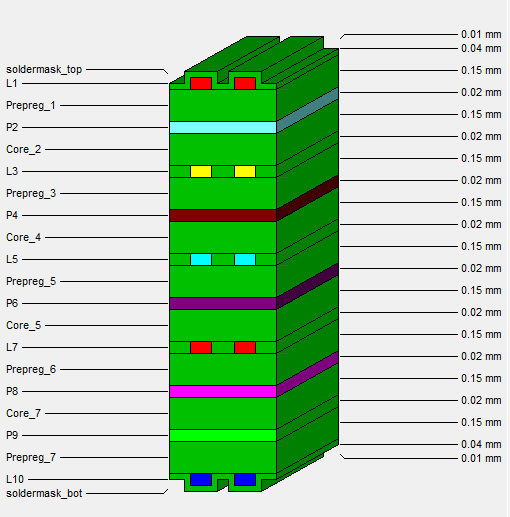
\includegraphics[width=12cm]{img/stackup.png}\\
		\caption{SAYMA RTM stackup}
	\end{figure}
	
\textit{\textbf{Note:}The thickness of copper in Figure 17 is 0.04mm and 0.02mm is due to approximation. In fact it is 0.036mm and 0.018mm.}	